\documentclass{article}
\usepackage[preprint]{corl_2026}
\usepackage{amsmath}
\usepackage{graphicx}
\usepackage{booktabs}
\graphicspath{{../figures/paper/}}
\hypersetup{pdftitle={Tracking Error as an Observation for Behavior Cloning on Low-Cost Arms},
 pdfauthor={Luai Abuelsamen}, pdfsubject={Research preprint}}

\title{Tracking Error as an Observation for Behavior Cloning on Low-Cost Arms}
\author{Luai Abuelsamen\\University of California, Berkeley\\
\texttt{luai\_abuelsamen@berkeley.edu}}
\begin{document}
\maketitle

\begin{abstract}
Standard behavior-cloning stacks for low-cost arms observe one timestep of
joint positions. We show that appending the servo tracking error, the
difference between the last applied command and the measured position, changes
what a policy can learn at a 50-demonstration budget. On a physical SO-101, ACT
policies with tracking error place the object in 23 of 40 paired trials
against 6 of 40 for position-only policies (stratified exact test
$p=0.0005$), with the gain replicated across two training seeds. In simulation
over five seeds, placement rises from 6.2\% to 21.8\%, and a position-history
control recovers most of the gain, so the effect is attributable to temporal
information the default omits rather than to tracking error specifically. The
signal is free: it is reconstructible from existing logs, and it keeps varying
where the servo's load register saturates at a vendor torque limit in 16.5\% of
demonstration frames. Across 546 archived teleoperation episodes, tracking
error at grasp onset marks resistance but not grasp success, so it is an
observation, not an outcome label.
\end{abstract}
\keywords{Behavior Cloning, Proprioception, Low-Cost Manipulation}

\section{Introduction}
A position command describes an intended motion, and during manipulation the
gap between that command and the position actually reached can persist for many
steps---because a finger has met an object, because a joint is carrying a load,
or simply because the actuator has not caught up. A policy given only the
current joint position must infer all of this from its remaining observations,
whereas supplying the previous command makes the discrepancy directly
available.

Standard behavior-cloning stacks for low-cost arms observe a single timestep
of joint positions. Tracking error needs neither an added sensor nor a force
model, and it can be reconstructed from existing demonstrations wherever the
logged commands are the goals the servos received. It also mixes contact with
motion lag and actuator dynamics, and a history of positions may carry the same
information, so the question is whether exposing it helps an imitation policy,
and whether any gain is specific to it.

We run two experiments. A simulation grid sets explicit tracking error against
action history, position history and a compensated residual under identical
data and training budgets. A hardware study asks whether the simplest of these
features helps ACT policies trained on 50 human demonstrations on one SO-101.
On the arm, tracking error places 23 of 40 paired trials against 6 of 40,
replicated across two training seeds. In simulation, position history recovers
most of the gain, so the result is that the single-timestep default omits
temporal information a policy needs, and tracking error is the temporal
channel every existing log already contains.

\section{Related work}
Hwang et al.~\citep{hwang2018virtual} estimate torque on RC servos by system
identification; FACTR~2~\citep{oh2026factr2} learns external-torque estimates
from free-motion data and resamples training data by force. We use a simpler
input, the uncalibrated command--position difference, and make
correspondingly weaker claims about force.

Wong et al.~\citep{wong2026beyond} show that leader--follower discrepancies in
teleoperation can carry interaction cues: removing them from ACT's action
labels degrades performance in force-critical phases, while torque proxies
restore contact-aware behavior. Our intervention instead adds the discrepancy
to the policy observation, which makes this an observation-design study rather
than a new sensorless-force principle. Adding the feature also adds access to the
previous command. History that helps under partial observability can equally
support a shortcut that copies the previous action instead of the action the
task needs~\citep{wen2020copycat}, so we compare several temporal observations
rather than treating any gain over the base as evidence of force estimation.

\section{Observation and experimental design}
Let $q_t$ be the measured joint position and $g_{t-1}$ the preceding applied
position goal, expressed in the same coordinate system. We define
\begin{equation}
\delta_t = g_{t-1}-q_t,\qquad
 o_t^{\mathrm{base}}=[I_t,\widetilde q_t],\qquad
 o_t^{\delta}=[I_t,\widetilde q_t,\delta_t/c],
\end{equation}
where $I_t$ is the camera observation and $\widetilde q_t$ uses training-set
normalization. The scale $c=8$ is fixed in each dataset's joint-coordinate
units and is not a conversion to torque. Under approximately static contact,
tracking error may reflect load on a position servo, but during motion it also
contains following error, so we use it as an observation without assigning
every nonzero value to external contact.

\textbf{Simulation.} We train ACT policies~\citep{zhao2023act} on 280 scripted
pick-and-place demonstrations with randomized object and scene properties.
All designs use the same data and training budget: 12,000 steps with 96-pixel
front and gripper-camera images. Each trained policy is evaluated on 100
episodes with shared scene seeds across designs, with five training seeds for
the original designs and three for the position-history control.
The learning comparison uses placement success with the crush threshold
disabled, so it tests grasping and transport rather than regulation within a
safe force band.

\textbf{Hardware.} We collect 50 teleoperated demonstrations of placing an
adapter inside a tape roll using one SO-101 and one overhead camera. Both
policies use the same 18,549 training frames after removal of stationary
prefixes, 96-pixel images, and 6,000 training steps. The proprioceptive input
has six dimensions for the base and twelve for tracking error; all other
architecture and optimization settings are shared. Three seeds are trained, one
checkpoint per observation design and seed.

Evaluation begins after replaying 115 commands from a fixed demonstration,
which places the arm near the grasp, after which each policy controls up to 400
steps. In the demonstrations the grasp closure occurs at a median frame 331 of
a median 400-frame episode and after frame 115 in 48 of 50 episodes, and a
median 67\% of joint travel follows frame 115, so the replay covers the
approach and leaves the grasp to the policy (Appendix~\ref{app:traces}). ACT predicts and executes 30-command chunks, so observations inform the
next chunk rather than each command within it. A relative-target limiter is
shared by both policies, and the tracking-error input uses the command returned
\emph{after} limiting. Trials are paired by training seed and physical reset,
with base-first and tracking-error-first order alternating across pairs, and
an operator records whether the adapter is placed inside the roll
(Appendix~\ref{app:protocol}).

\section{Results}
\begin{figure}[t]
\centering
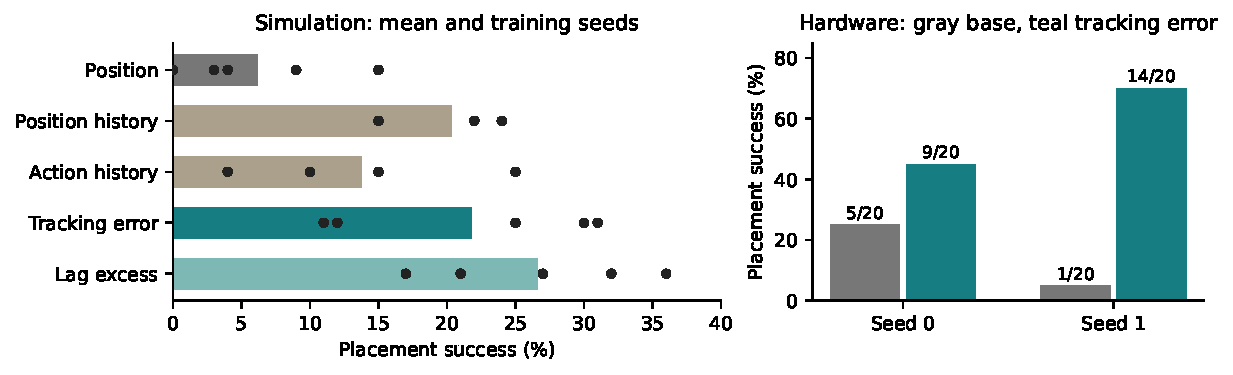
\includegraphics[width=\linewidth]{fig_observation_evidence.pdf}
\caption{Placement success by observation design in simulation and in the two
completed hardware evaluations. Left: bars are means; dots are
individual training seeds (five per design, three for position history).
Right: hardware success counts for the two completed evaluations. The full
evaluation record, including an interrupted third comparison, appears in
Appendix~\ref{app:protocol}.}
\label{fig:evidence}
\end{figure}

\begin{figure}[t]
\centering
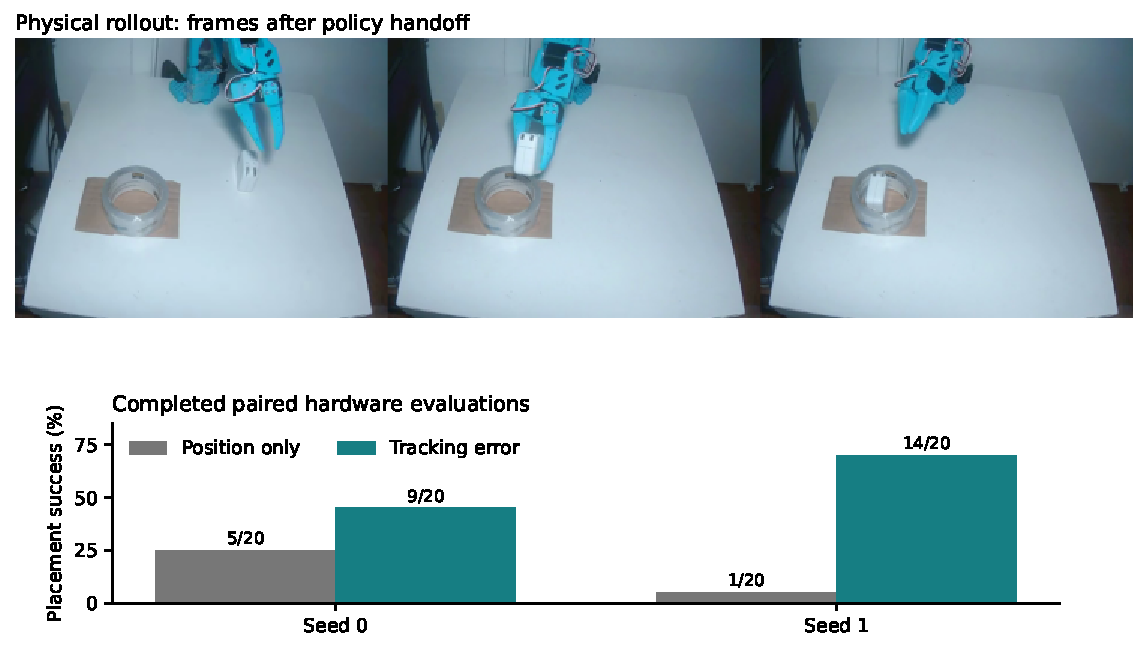
\includegraphics[width=\linewidth]{fig_real_quantitative.pdf}
\caption{Top: three frames from a tracking-error policy (seed 1) after the
scripted replay, from a showcase rollout that is not included in any count.
Bottom: placement successes over 20 pairs for the two completed hardware
evaluations.}
\label{fig:real}
\end{figure}

In simulation, temporal information helps and its best representation is
unresolved. Mean placement success is 6.2\% for the position-only base,
13.8\% with the previous action appended, and 21.8\% with explicit tracking
error. A compensated residual reaches 26.6\%, while position history alone
reaches 20.3\% (Fig.~\ref{fig:evidence}). Tracking error exceeds the base by
15.6 points (Welch 95\% CI 3.5 to 27.7) and position history by 1.5 points
(CI $-11.1$ to 14.0); position history itself exceeds the base by 14.1 points
(CI 4.5 to 23.8). Only the tracking-error and compensated-residual gains over
the base clear the preregistered resolution rule of $15\sqrt{3/n}$ points for
$n$ seeds (Appendix~\ref{app:sim}). Because the residual subtracts a
fitted free-motion term from tracking error and uses two previous commands,
comparing it against one-command history changes both the information available
and its representation. Position history recovers most of the gain without
observing commands at all, so what the grid identifies is the cost of the
single-timestep default, not a property of tracking error specifically. Predicting tracking error as an
auxiliary training target gives 6.6\%: this particular auxiliary objective does
not recover the benefit of supplying it as input.

On hardware, tracking error places 23 of 40 against 6 of 40 across the two
completed seeds. Table~\ref{tab:hardware} reports each comparison separately:
9/20 against 5/20 for seed 0 and 14/20 against 1/20 for seed 1, improvements
of 20 and 65 percentage points. Exact two-sided McNemar
tests use only the discordant pairs. Seed 0 has six pairs favouring tracking
error and two favouring the base ($p=0.29$); seed 1 has fourteen and one
($p=0.001$). The first comparison is inconclusive and the second is not. Both
tests describe trial-to-trial variation for a fixed pair of checkpoints, not
variation over training seeds. Pooling the completed seeds gives 20 discordant
pairs favouring tracking error against 3 (stratified exact test $p=0.0005$;
conditional odds ratio 6.7, 95\% CI 2.0 to 35), and the two discordance
ratios are not detectably different (Fisher $p=0.27$); these pooled figures
still condition on two checkpoint pairs and are not an estimate over
retraining. With 20 pairs the exact test has power 0.17 under seed 0's
observed discordance structure and 0.97 under seed 1's, so the protocol could
detect only large effects (Appendix~\ref{app:protocol}). Offline, all three
tracking-error checkpoints depend on the tracking-error input: zeroing it
changes the predicted jaw command by 12.6 to 13.0 units on frames where the
gripper load register is at its limit and by 2.7 to 2.9 units elsewhere,
against a median recorded command step of 0.5. Teacher-forcing error on the
training frames separates the designs, 2.9 to 3.6 for tracking error against
3.7 to 3.9 for the base, but does not order the two tracking-error checkpoints
as the hardware did (Appendix~\ref{app:sensitivity}).

\begin{table}[t]
\centering
\small
\caption{Hardware placements and paired outcomes for the two completed evaluations.
Discordances list tracking-error-only / base-only successes. See
Appendix~\ref{app:protocol} for the interrupted evaluation.}
\label{tab:hardware}
\begin{tabular}{llrrrr}
\toprule
Seed & Evaluation & Base & Tracking error & Discordances & $p$ \\
\midrule
0 & Complete & 5/20 & 9/20 & 6 / 2 & 0.2891 \\
1 & Complete & 1/20 & 14/20 & 14 / 1 & 0.0010 \\
\bottomrule
\end{tabular}

\end{table}

A third evaluation was interrupted by recurring hardware faults; its partial
results and missing outcomes are reported in Appendix~\ref{app:protocol}.

The shipped force signal is clipped. The follower's gripper load register sits
at its configured torque limit of 500 in 16.5\% of demonstration frames and
touches it in every episode, while tracking error keeps varying on those
frames; over all frames the two correlate at $r=-0.92$
(Appendix~\ref{app:measure}). A vendor default therefore removes the only
shipped force telemetry exactly where the jaw is loaded, and the
command--position discrepancy is the signal that survives it.

A useful input is not necessarily an outcome label. We also test a
preregistered prediction that larger tracking error at detected grasp onset
accompanies successful grasps in archived teleoperation data. Sixteen datasets
with 546 episodes pass the inclusion gates, of which only two meet the
predicted positive effect-size threshold ($d>0.5$); the pooled within-dataset
effect is negative ($d=-0.39$), scored against a gripper-retention proxy, not
manually verified placements. The result rejects this proposed labeling rule
and illustrates why a discrepancy can indicate resistance without identifying a
successful grasp (Appendix~\ref{app:corpus}).

\section{Discussion and conclusion}
Behavior-cloning stacks for low-cost arms default to a single timestep of
joint positions, and at a 50-demonstration budget that default is the limiting
choice. Adding the servo tracking error raised placements on a physical SO-101
from 6 of 40 to 23 of 40 across two training seeds, and in simulation from
6.2\% to 21.8\% over five. Position history recovers most of the simulated
gain without observing commands, so the finding is that the default omits
temporal information a policy needs and any temporal channel repairs it.
Tracking error is the channel every existing log already contains, and it
keeps varying where the vendor-limited load register saturates.

Three limitations bound the claim. The hardware effect differs across seeds,
20 and 65 points, and two completed seeds cannot bound that spread. A matched
position-history control on hardware is registered but not yet evaluated
(Appendix~\ref{app:history}), so whether tracking error adds anything beyond
history on the arm is open. The task never requires staying under a force
limit, so nothing here shows learned force regulation, and the corpus study
shows tracking error marks resistance, not success. The study covers one arm,
one task and a fixed scripted approach.

The next experiments are the registered hardware history control, more
training seeds per design, and a task with a measured force limit.

\clearpage
\bibliography{refs}
\clearpage
\appendix

\section{Hardware protocol and complete evaluation record}
\label{app:protocol}
\begin{table}[h]
\centering
\small
\caption{Full hardware evaluation record: success counts with Wilson 95\%
intervals in percentage points, discordant and concordant pair counts, exact
McNemar $p$ per seed, and the stratified exact test over the completed seeds.
The interrupted seed has six recorded pairs, with 0/6 placements for each
policy; its planned budget was 20 pairs. No confirmatory test is assigned to
the incomplete comparison.}
\resizebox{\linewidth}{!}{\begin{tabular}{llllrrr}
\toprule
Seed & Evaluation & Base (Wilson 95\%) & Tracking error (Wilson 95\%) & TE-only / base-only & both / neither & $p$ \\
\midrule
0 & Complete & 5/20 [+11, +47] & 9/20 [+26, +66] & 6 / 2 & 3 / 9 & 0.2891 \\
1 & Complete & 1/20 [+1, +24] & 14/20 [+48, +85] & 14 / 1 & 0 / 5 & 0.0010 \\
2 & Interrupted & 0/6 [+0, +39] & 0/6 [+0, +39] & 0 / 0 & 0 / 6 & --- \\
\midrule
Stratified (completed) & & & & 20 / 3 & & 0.0005 \\
\bottomrule
\end{tabular}
}
\end{table}

\begin{table}[h]
\centering
\small
\caption{Power of the exact two-sided McNemar test with 20 pairs at
$\alpha=0.05$, by the probability that a pair is discordant and the probability
$q$ that a discordant pair favours tracking error. Seed 0's observed structure
(8 discordant pairs, 6 favouring) gives 0.17; seed 1's (15, 14) gives 0.97.}
\label{tab:power}
\begin{tabular}{lrrrr}
\toprule
P(discordant) & $q=0.7$ & $q=0.8$ & $q=0.9$ & $q=1.0$ \\
\midrule
0.2 & 0.02 & 0.05 & 0.10 & 0.20 \\
0.4 & 0.11 & 0.26 & 0.53 & 0.87 \\
0.6 & 0.19 & 0.46 & 0.80 & 1.00 \\
0.8 & 0.29 & 0.64 & 0.93 & 1.00 \\
\bottomrule
\end{tabular}

\end{table}

\textbf{Training.} The recording contains 21,476 frames from 50 demonstrations
at 30\,Hz. Position and action statistics are computed on the recording; the
training index then removes stationary prefixes, retaining 18,549 frames. Both
policies use the same index and normalization, and recorded load channels are
excluded from policy inputs. Gripper position is in the interface's own units,
not a calibrated force.

The ACT configuration uses a ResNet-18 image backbone, model width 256,
four attention heads, feedforward width 1024, two encoder layers and one
decoder layer. The action chunk and execution horizon are both 30 steps,
with no temporal ensembling. Optimization uses AdamW at learning rate
$10^{-4}$, weight decay $10^{-4}$, batch size 8 and gradient clipping at 10.
All reported checkpoints are the final checkpoint at 6,000 steps. The
observation projection necessarily changes width when six features are added;
the remaining architecture and training settings are shared.

\textbf{Execution and command semantics.} Each rollout homes the arm to the
mean demonstration start, replays the first 115 commands from demonstration 0,
and hands control to the policy, so the reported task excludes autonomous
approach from an arbitrary initial state. Each requested command passes through
a relative-target limit of 8 in the interface's joint units---a
target-displacement bound rather than a force or velocity guarantee---and
during both replay and policy execution the returned limited command supplies
the next tracking-error calculation. The servo's native goal quantization sits
below this software interface. State and images are read at each control step,
but ACT consults them only when its 30-command queue is empty.

An offline replay check reproduces the training and inference state vectors
on all 21,476 recorded frames for the base, tracking error, action history,
position history and compensated residual designs. In seed 0, the saved
tracking-error observations after the first rollout step also reproduce from
logged applied commands, which checks software consistency, not physical
command-to-encoder latency. Collection-time command limiting has not been
established from the available metadata, so archived action labels should be
read as recorded goals, which need not equal the goals applied to a servo if
collection used an additional limiter.

\textbf{Pairing and inference.} Hardware resets are manual, and within each
seed consecutive trials form a pair with AB/BA order alternating between pairs.
The operator knows the policy identity, so outcomes are not blinded. Outcomes
show no order effect: seed-1 tracking error placed 7/10 whether it ran first
or second in a pair and in both halves of the session, and seed 0 placed 5/10
and 4/10 by order and 3/10 and 6/10 by half. Seeds 1
and 2 were scheduled after observing seed 0, with their training recipe and
evaluation budget fixed before their evaluations, and no policy was selected by
hardware performance: every trained checkpoint was evaluated. The primary paired test is exact, two-sided McNemar with
an improvement criterion of positive effect and $p<0.05$; for the completed
seeds, paired percentile bootstrap intervals (20,000 pair resamples, random
seed 0) are $[-5,+45]$ and $[+40,+90]$ points, describing trial uncertainty
for fixed checkpoints, not confidence intervals over retraining.

\textbf{Interruptions and missing data.} Seed 0 has 40 outcomes and 40
trajectories. Seed 1 has 40 outcomes and 39 trajectories: two rollouts, one per
policy, completed their control horizon but reported a gripper overload while
torque was being disabled; both are operator-labeled failures, and one
trajectory file was lost to a logging bug that was fixed before evaluation
resumed. Seed 2 was stopped after twelve labeled rollouts, all failures,
forming six pairs; three reported the same overload at shutdown, and a
thirteenth rollout completed its horizon but its outcome was not entered. We
leave that outcome missing rather than infer it from joint motion, and we have
no diagnosis of the recurring overload. In the seed-2 rollouts the jaw never
closed in five of six position-only and three of six tracking-error trials,
against three of 20 and one of 20 in seed 0 and two of 20 and none of 19 in
seed 1 (Table~\ref{tab:traces}), which is consistent with a gripper fault
rather than a policy difference, although the traces cannot prove it.
Trial-level detail is in the repository's evaluation records.

\section{Exploratory trajectory analysis}
\label{app:traces}
\begin{figure}[t]
\centering
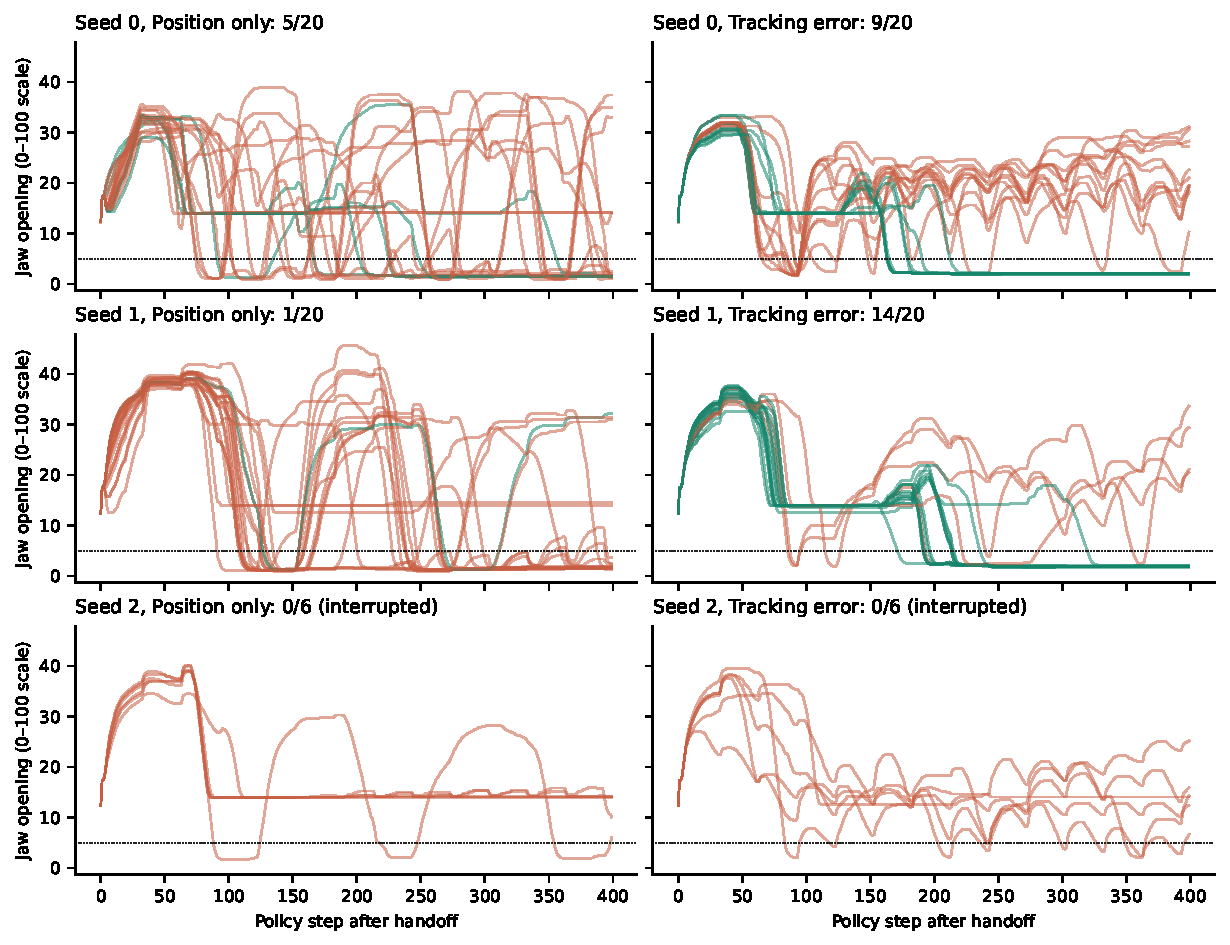
\includegraphics[width=\linewidth]{fig_hardware_traces.pdf}
\caption{Recorded jaw position for every hardware rollout, by seed and
policy; green traces placed the adapter, orange did not. Policy control
begins at step 0 after the scripted replay. The dotted line marks the closure
threshold used in Table~\ref{tab:traces}.}
\label{fig:traces}
\end{figure}
\begin{table}[h]
\centering
\caption{Jaw-trace classes for all recorded rollouts. Never closed: jaw never
below 5 recorded units. Reopened: an excursion above 8 units after closing.
Closure step is the median first step below the threshold. One seed-1
tracking-error trajectory is missing.}
\label{tab:traces}
\resizebox{\linewidth}{!}{\begin{tabular}{lllrrrrr}
\toprule
Seed & Policy & Outcome & $n$ & never closed & closed, reopened & closed, held & median step of closure \\
\midrule
0 & Position only & success & 5 & 0 & 1 & 4 & 203 \\
0 & Position only & failure & 15 & 3 & 8 & 4 & 110 \\
0 & Tracking error & success & 9 & 0 & 0 & 9 & 165 \\
0 & Tracking error & failure & 11 & 1 & 10 & 0 & 83 \\
1 & Position only & success & 1 & 0 & 1 & 0 & 127 \\
1 & Position only & failure & 19 & 2 & 13 & 4 & 116 \\
1 & Tracking error & success & 14 & 0 & 0 & 14 & 206 \\
1 & Tracking error & failure & 5 & 0 & 4 & 1 & 115 \\
2 & Position only & failure & 6 & 5 & 1 & 0 & 88 \\
2 & Tracking error & failure & 6 & 3 & 3 & 0 & 241 \\
\bottomrule
\end{tabular}
}
\end{table}
Every recorded rollout was classified from its jaw trace as never closed,
closed then reopened, or closed and held (Table~\ref{tab:traces},
Fig.~\ref{fig:traces}). All 23 tracking-error successes in seeds 0 and 1
closed once and held to the end of the horizon, and 15 of their 16 failures
either never closed or reopened. Position-only successes are too few to
characterize. Successful tracking-error rollouts closed later, at median step
165 and 206 against 83 and 115 for failures, and in seed 0 they requested
smaller moves: the median fraction of steps altered by the command limiter is
0.09 for tracking error and 0.32 for the base, while in seed 1 the fractions
are 0.32 and 0.35. Over the last 100 steps of the seed-0 tracking-error
rollouts, median summed joint-coordinate travel, a descriptive sum over mixed
coordinates, is 14.3 for successes and 93.6 for failures. Later closure and
less motion in successful trials could simply follow from progressing further
through the task. Traces were grouped by outcome after the fact and contain no
video, object pose or force, so they cannot say whether a failure was a missed
grasp, a slip or a misplacement, and none of these regularities is a validated
success detector. In tracking-error rollouts the median absolute jaw tracking
error after closure is 0.11 and 0.16 units for successes and 1.04 and 0.88 for
failures (seeds 0 and 1): a held grasp settles to a small steady discrepancy,
whereas reopening and re-closing keeps it large. Fig.~\ref{fig:timing} shows
when the jaw first closes in each rollout and, for the demonstrations, when
the grasp closure occurs relative to the replayed prefix.

\begin{figure}[h]
\centering
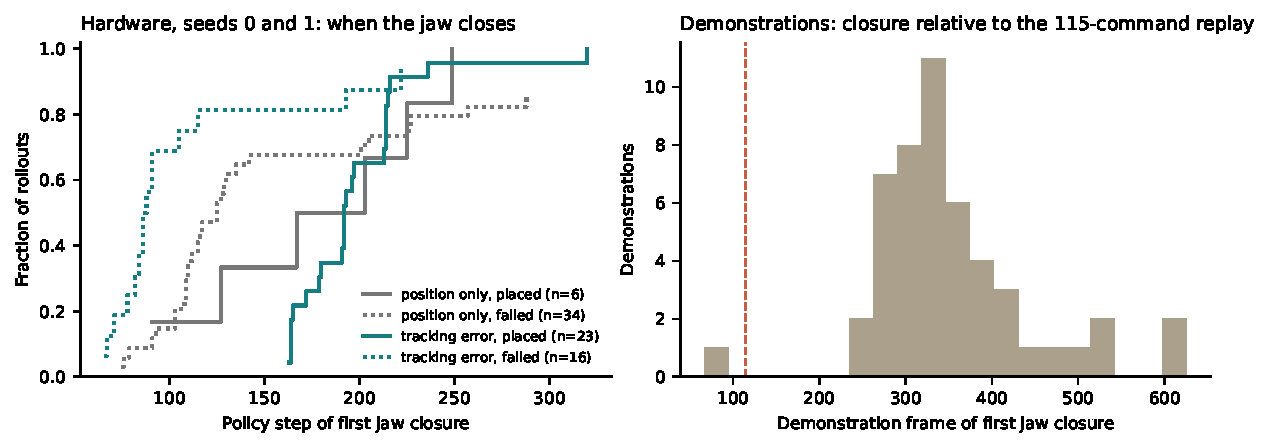
\includegraphics[width=\linewidth]{fig_timing.pdf}
\caption{Left: cumulative fraction of hardware rollouts (seeds 0 and 1) whose
jaw has closed by a given policy step, by policy and outcome. Right: frame of
the grasp closure in the 50 demonstrations; the dashed line is the 115-command
replay.}
\label{fig:timing}
\end{figure}

\section{Checkpoint sensitivity and offline error}
\label{app:sensitivity}
\begin{figure}[h]
\centering
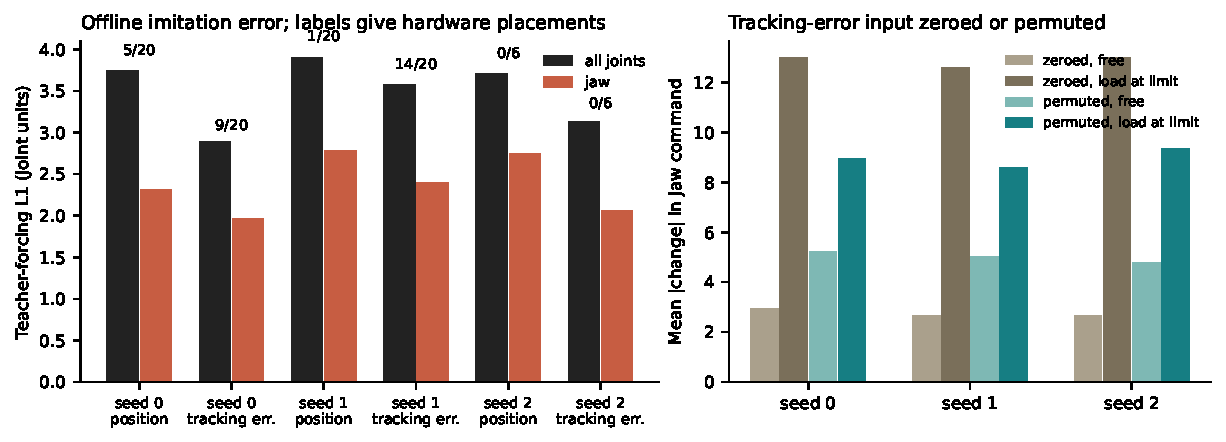
\includegraphics[width=\linewidth]{fig_sensitivity.pdf}
\caption{Left: teacher-forcing L1 error of each evaluated checkpoint's
predicted 30-command chunk on every fourth training frame (4,638 frames), all
joints and jaw; labels give hardware placements. Right: mean absolute change
in the predicted jaw command when the six tracking-error inputs are zeroed or
permuted across frames, split by whether the recorded gripper load register is
at its limit (881 frames) or not.}
\label{fig:sensitivity}
\end{figure}
The hardware trials cannot say whether a policy reads its tracking-error
input, so the six evaluated checkpoints were re-scored offline on the
demonstration frames (Fig.~\ref{fig:sensitivity}). Zeroing the input changes
the predicted jaw command by 12.6 to 13.0 units where the load register is
pinned and by 2.7 to 2.9 units on free frames; permuting it across frames
changes the command by 8.6 to 9.4 and 4.8 to 5.2 units. The median recorded
command step is 0.5 units, and teacher-forcing error rises from 2.9 to 3.6 to
6.2 to 6.8 under zeroing. All three tracking-error checkpoints therefore
depend on the channel, most where the jaw is loaded; this is a property of the
networks, not evidence that the dependence is what produced the hardware
placements. Offline error itself is a fit diagnostic on training frames, since
no demonstrations were held out: it separates designs but ranks the seed-0
tracking-error checkpoint (2.9, 9/20) below the seed-1 checkpoint (3.6,
14/20). Training losses of the seed-1 and seed-2 checkpoints track each other
closely (Fig.~\ref{fig:training}).

\begin{figure}[h]
\centering
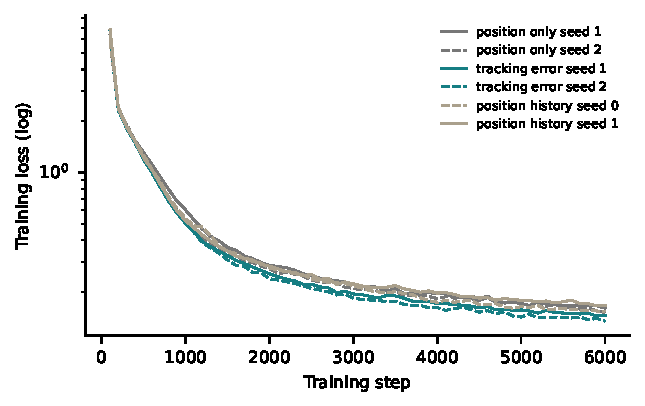
\includegraphics[width=.6\linewidth]{fig_training.pdf}
\caption{Training loss, logged every 100 steps, for the checkpoints whose logs
are in the repository.}
\label{fig:training}
\end{figure}

\section{The shipped load register saturates at a vendor limit}
\label{app:measure}
A separate static experiment on one shoulder-lift STS3215 uses twelve hanging
masses
at five poses (60 measurements). Across those measurements, the fitted
relationship between the load register and tracking error is
$\texttt{Present\_Load}=-4.70\delta+0.1$, with $R^2=0.976$.
Its relation to applied mass is far less stable, with per-pose $R^2$ for
tracking error ranging from 0.085 to 0.910, so the tight load-register
association does not establish an equally accurate physical-load measurement.

In the 50 teleoperation demonstrations, the gripper load register reaches
500 in every episode and remains there in 16.5\% of frames, while tracking
error continues to vary across those same frames (Fig.~\ref{fig:measurement});
over all frames the two channels correlate at $r=-0.92$. The inspected follower
configuration sets a reduced gripper torque limit, consistent with that
observed plateau. This motivates inspecting the command--position discrepancy
when telemetry saturates, but it does not calibrate the remaining discrepancy
in newtons: no jaw load-cell calibration is available, and simulator force
conversions such as the fitted 2.00\,N/count slope and 4.3\,N held-out RMSE
over 4--78\,N describe the simulated plant only.

\section{Simulated plant}
\label{app:plant}
The simulated plant was characterised with scripted experts before any policy
was trained, to check that tracking error can carry contact information in
this simulator at all. Three experts differ only in the signal that sets the
grip: a fixed jaw angle (clamp), the quantised tracking error, or the true
contact force (oracle). Without a crush limit the clamp places 29 of 30 and
the two regulated experts 22 and 20, because a gentler grip drops more often
and nothing penalises crushing. With a crush limit the clamp fails every
episode at a median peak grip of 355\,N, while the tracking-error expert at
the native quantum places within a few episodes of the oracle at every limit,
and coarsening the observation quantum destroys the task as a cliff whose
position moves with the margin (Table~\ref{tab:plant}). This is why the
learning grid could ask whether a policy uses the channel: in this plant the
channel suffices for force regulation by a scripted controller at the real
encoder's resolution. It does not show that the physical servo provides the
same information; Appendix~\ref{app:measure} addresses that separately.

\begin{table}[h]
\centering
\small
\caption{Scripted-expert placements out of 30 randomised episodes in the
simulated plant, by grip signal and observation quantum, with and without a
crush limit that fails the episode if grip force exceeds it.}
\label{tab:plant}
\begin{tabular}{lrrrrrrr}
\toprule
 & \multicolumn{5}{c}{tracking error, quantum $q$ (counts)} & clamp & oracle \\
Crush limit & 1 & 4 & 8 & 16 & 32 & & \\
\midrule
no limit & 22 & --- & --- & --- & --- & 29 & 20 \\
100\,N & 11 & 11 & 9 & 1 & 0 & 0 & 12 \\
120\,N & 17 & 17 & 16 & 10 & 0 & 0 & 14 \\
160\,N & 20 & 20 & 19 & 17 & 11 & 0 & 17 \\
\bottomrule
\end{tabular}

\end{table}

\begin{figure}[t]
\centering
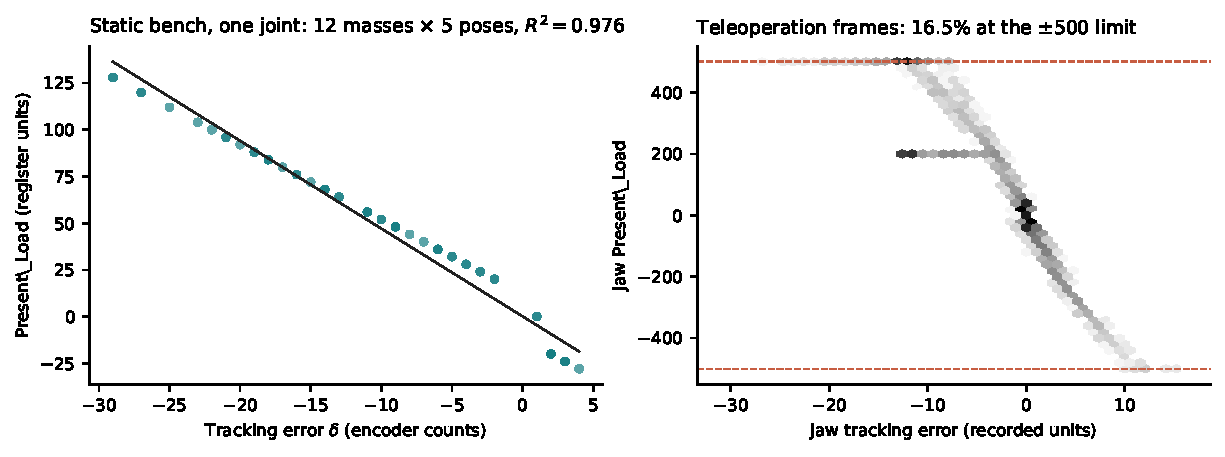
\includegraphics[width=\linewidth]{fig_measurement.pdf}
\caption{Left: static bench, one shoulder-lift servo, load register against
tracking error over twelve hanging masses at five poses, with the fitted line.
Right: jaw load register against jaw tracking error on the teleoperation
frames (log-count shading); the dashed lines are the configured $\pm500$
torque limit.}
\label{fig:measurement}
\end{figure}

\section{Additional simulation and hardware comparisons}
\label{app:sim}
Simulation recordings use integer encoder counts at 15\,Hz, obtained by
subsampling the 30\,Hz controller. The scripted teacher regulates the jaw
using tracking error, and the successful demonstration set includes randomized
grip depth and recovery perturbations. These collection choices are shared
across observation designs, of which the position-history control observes
$[q_t,q_{t-8}]$ and one-command history observes $[q_t,g_{t-1}]$. Neither
comparison makes the simulation and hardware tasks identical: camera views,
demonstrations and recording cadence all differ between the two settings.

The original simulation study includes an auxiliary tracking-error target
and a latched seat token in addition to the designs in
Fig.~\ref{fig:evidence}, with mean placement rates of 6.6\% and 21.8\% across
five seeds; the seat token matches tracking error exactly. The compensated residual is
$e_t=\delta_t-\widehat K(g_{t-1}-g_{t-2})$, where each joint's coefficient
is fitted once on presumed free-motion demonstration frames. A two-command
history control reaches 14.7\% over three seeds; comparing it with the residual
holds available raw information fixed but does not match input width. Under the
original study's preregistered practical resolution rule, $15\sqrt{3/n}$
percentage points for $n$ training seeds, neither this comparison nor the
residual--position-history comparison resolves at three seeds, and the stronger
feature-specific interpretation remains open. Table~\ref{tab:contrasts} lists
the main design contrasts with Welch intervals; the Holm column adjusts across
all 28 pairwise comparisons, and no contrast survives that adjustment. The
preregistered contrasts against the base are the primary tests; the adjustment
across every pair is reported for completeness.

\begin{table}[h]
\centering
\caption{Simulation design contrasts in placement-success points, with Welch
95\% intervals, unadjusted and Holm-adjusted $p$ values across all 28 pairs,
the preregistered resolution rule $15\sqrt{3/n}$ for the smaller seed count,
and whether the difference clears it.}
\label{tab:contrasts}
\resizebox{\linewidth}{!}{\begin{tabular}{lrlrrrl}
\toprule
Contrast & Points & Welch 95\% CI & $p$ & Holm $p$ & Rule & Clears \\
\midrule
Position history $-$ Position & +14.1 & [+4.5, +23.8] & 0.013 & 0.33 & 15.0 & no \\
Action history $-$ Position & +7.6 & [-2.5, +17.7] & 0.121 & 1.00 & 11.6 & no \\
Tracking error $-$ Position & +15.6 & [+3.5, +27.7] & 0.019 & 0.44 & 11.6 & yes \\
Compensated residual $-$ Position & +20.4 & [+10.2, +30.6] & 0.002 & 0.05 & 11.6 & yes \\
Auxiliary target $-$ Position & +0.4 & [-7.1, +7.9] & 0.903 & 1.00 & 11.6 & no \\
Tracking error $-$ Position history & +1.5 & [-11.1, +14.0] & 0.784 & 1.00 & 15.0 & no \\
Compensated residual $-$ Position history & +6.3 & [-4.6, +17.1] & 0.206 & 1.00 & 15.0 & no \\
Tracking error $-$ Action history & +8.0 & [-4.9, +20.9] & 0.188 & 1.00 & 11.6 & no \\
Compensated residual $-$ Two-command history & +11.9 & [+2.2, +21.7] & 0.025 & 0.49 & 15.0 & no \\
Compensated residual $-$ Tracking error & +4.8 & [-8.1, +17.7] & 0.413 & 1.00 & 11.6 & no \\
\bottomrule
\end{tabular}
}
\end{table}

An earlier hardware comparison, run before the tracking-error study, evaluated the
compensated residual: the base placed 7/10 objects and the residual 0/10
(Fisher exact $p=0.003$; Wilson intervals 40 to 89\% and 0 to 28\%;
alternating unpaired trials with the same 115-command replay). The
coefficients fitted from these real demonstrations differ markedly from the
simulation fits, and a free-motion labeling heuristic includes contact frames.
Both are plausible sources of mismatch, not a diagnosis. Coefficients above
one do not by themselves invalidate the regression, and that runner also fed
back requested rather than post-limit commands, so preprocessing and execution
both differ from the tracking-error study.

The simulation task admits a crush threshold, but the learning grid does not
activate it. A post-hoc screen of existing checkpoints at 120 and 60\,N
produces heavy crushing and near-floor success, failing the predicted
advantage of the compensated residual. A separate runtime guard reduces crush
events from 85 to 3 across 180 crush-tier episodes, while eliminating all
12 unguarded placements across its broader 270-episode comparison. Neither
result is learned force regulation, and the guard was not used on hardware.

Larger-budget experiments do not establish a scaling advantage. An earlier
600-demonstration comparison of tracking error and one-command history
reaches 57\% and 60\%, respectively, over two seeds at 224 pixels and 50,000
steps. A later 600-demonstration screen saved at 26,000 steps contains three
base and three residual evaluations, each with 0/100 placements. These
floor results are reported separately from the 280-demonstration grid; they
support neither a positive scaling claim nor equivalence between
observations.

\section{Archived teleoperation study}
\label{app:corpus}
The preregistered corpus prediction was that tracking error at a detected
seat event would be larger in proxy-successful episodes, with Cohen's
$d>0.5$ in at least ten of twenty targeted datasets. Sixteen datasets and 546
episodes pass the frozen gates, including 283 proxy successes under a success
proxy of continued gripper closure through transport. Only two datasets exceed
the positive threshold, and the pooled within-dataset effect is
$d=-0.39$---a failure of the proposed direction and labeling rule, though not
proof that no function of command and position history can predict outcome.
Eleven of the sixteen point estimates are negative and seven of those
intervals exclude zero; two are positive with intervals excluding zero
(Fig.~\ref{fig:corpus}).

\begin{figure}[h]
\centering
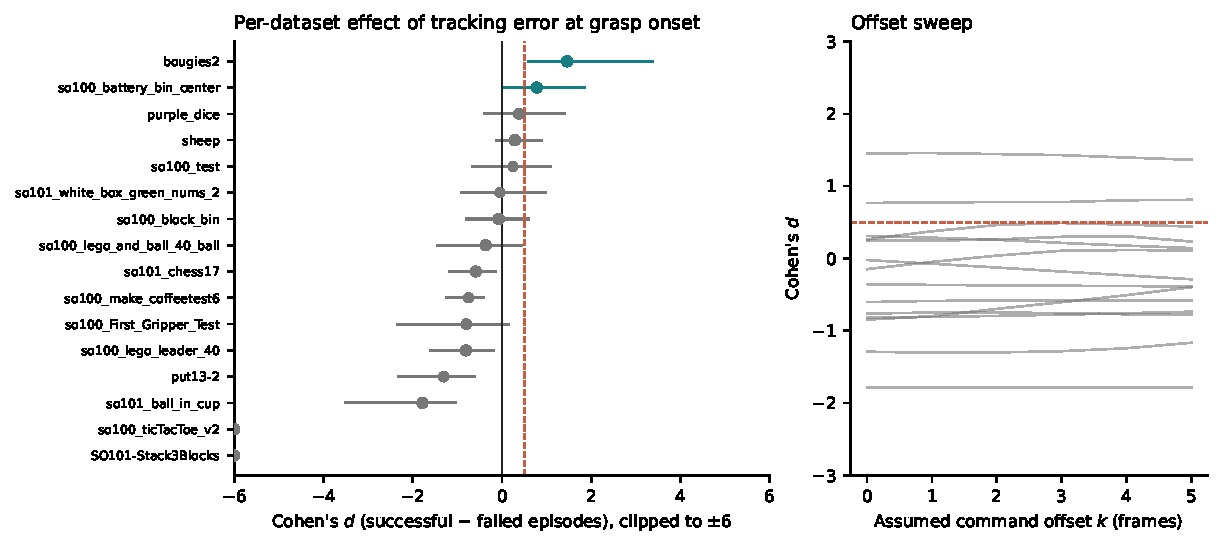
\includegraphics[width=\linewidth]{fig_corpus.pdf}
\caption{Left: per-dataset Cohen's $d$ of tracking error at grasp onset
between proxy-successful and failed episodes, with 95\% intervals, clipped to
$\pm6$; marker area scales with episode count and the dashed line is the
preregistered $d=0.5$ threshold. Right: the same effect sizes under assumed
command offsets of zero to five frames.}
\label{fig:corpus}
\end{figure}

Empty closure against a mechanical stop and closure on an object can both
produce a seat event, and a large command discrepancy can equally reflect an
operator continuing to close against resistance. These ambiguities explain why
a contact-related feature need not be a success label, although the corpus does
not isolate their causal contributions. Recorded leader commands may differ
from applied follower goals and the timing is only approximately aligned, but
an offset sweep from zero to five recorded frames leaves the qualitative
conclusion unchanged, with median per-dataset effect-size shift 0.12.

\section{Position-history control on hardware}
\label{app:history}
The simulation grid leaves open whether the hardware gain from tracking error
is specific to the command or would follow from any temporal input. A matched
position-history control, $[q_t, q_{t-8}]$ with the seed-1 and seed-2 training
recipe, is pre-registered in the repository together with the two paired
comparisons that would settle it: tracking error against position history for
seed 1, and position only against position history for seed 0, each with 20
pairs under the protocol of Appendix~\ref{app:protocol}.
At the time this version was built, the matched position-history checkpoints had not finished training. The comparison is registered in the repository and its results table is generated from the trial records when they exist; nothing here is hand-typed.


\begin{table}[h]
\centering
\small
\caption{Pre-registered position-history comparisons on hardware. Generated
from the trial records; empty until the trials exist.}
\label{tab:history}
\begin{tabular}{lllrrrrr}
\toprule
Seed & Comparison (A vs.\ B) & Session & A & B & B-only / A-only & $p$ & overloads \\
\midrule
1 & Tracking error vs.\ position history & Interrupted & 1/9 & 0/9 & 0 / 1 & 1.0000 & 4 \\
\bottomrule
\end{tabular}

\end{table}

\end{document}
